\documentclass[12pt,border=12pt]{standalone}
\usepackage[utf8]{inputenc}
\usepackage[utf8]{vietnam}

\usepackage{amsmath}
\usepackage{amsfonts}
\usepackage{amssymb}

\usepackage{tikz}
\usetikzlibrary{arrows, decorations.markings, calc, fadings, decorations.pathreplacing, patterns, decorations.pathmorphing, positioning}
\tikzset{middlearrow/.style={
    decoration={markings,
    mark= at position 0.5 with {\arrow{#1}},
    },
    postaction={decorate}
    }
}


\begin{document}
    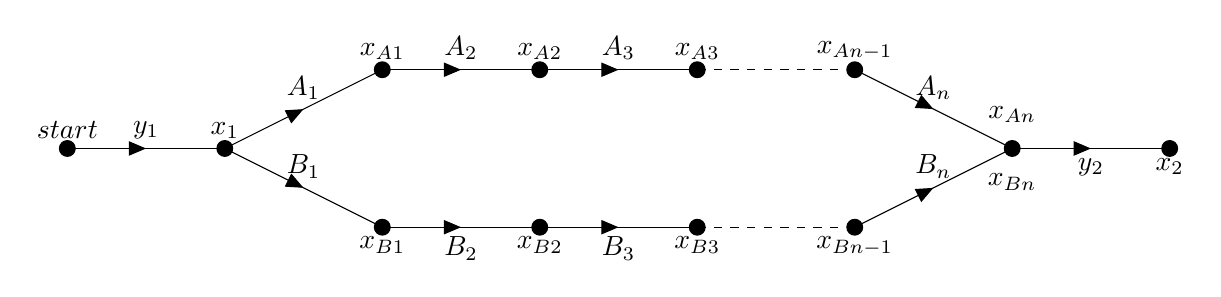
\begin{tikzpicture}[>=triangle 45]
        \draw[fill = black] (0, 0) circle (0.1) node[above] {$start$};
        \draw[middlearrow={>}] (0, 0) -- (2,0);
        \draw (1, 0) node[above] {$y_1$};
        \draw[fill = black] (2, 0) circle (0.1) node[above] {$x_1$};
					
        \draw[middlearrow={>}] (2, 0) -- (4, 1);
        \draw (3, 0.5) node[above] {$A_1$};
        \draw[fill = black] (4, 1) circle (0.1) node[above] {$x_{A1}$};
					
        \draw[middlearrow={>}] (4, 1) -- (6, 1);
        \draw (5, 1) node[above] {$A_2$};
        \draw[fill = black] (6, 1) circle (0.1) node[above] {$x_{A2}$};
        \draw[middlearrow={>}] (6, 1) -- (8, 1);
        \draw (7, 1) node[above] {$A_3$};
        \draw[fill = black] (8, 1) circle (0.1) node[above] {$x_{A3}$};
        \draw[dashed] (8, 1) -- (10, 1);
        \draw[fill = black] (10, 1) circle (0.1) node[above]{$x_{An-1}$};
        \draw[middlearrow={>}] (10, 1) -- (12, 0);
        \draw (11, 0.5) node[above] {$A_n$};
					
        \draw[middlearrow={>}] (2, 0) -- (4, -1);
        \draw (3, -0.5) node[above] {$B_1$};
        \draw[fill = black] (4, -1) circle (0.1) node[below] {$x_{B1}$};
					
        \draw[middlearrow={>}] (4, -1) -- (6, -1);
        \draw (5, -1) node[below] {$B_2$};
        \draw[fill = black] (6, -1) circle (0.1) node[below] {$x_{B2}$};
        \draw[middlearrow={>}] (6, -1) -- (8, -1);
        \draw (7, -1) node[below] {$B_3$};
        \draw[fill = black] (8, -1) circle (0.1) node[below] {$x_{B3}$};
        \draw[dashed] (8, -1) -- (10, -1);
        \draw[fill = black] (10, -1) circle (0.1) node[below]{$x_{Bn-1}$};
        \draw[middlearrow={>}] (10, -1) -- (12, 0);
        \draw (11, -0.5) node[above] {$B_n$};
        
        \draw[fill = black] (12, 0) circle (0.1);
        \draw (12, 0.2) node[above] {$x_{An}$};
        \draw (12, -0.2) node[below] {$x_{Bn}$};
        \draw[middlearrow={>}] (12, 0) -- (14, 0);
        \draw (13, 0) node[below] {$y_2$};
        \draw[fill = black] (14, 0) circle (0.1) node[below]{$x_2$};
    \end{tikzpicture}
\end{document}